\documentclass{standalone}
\usepackage{tikz}

\begin{document}
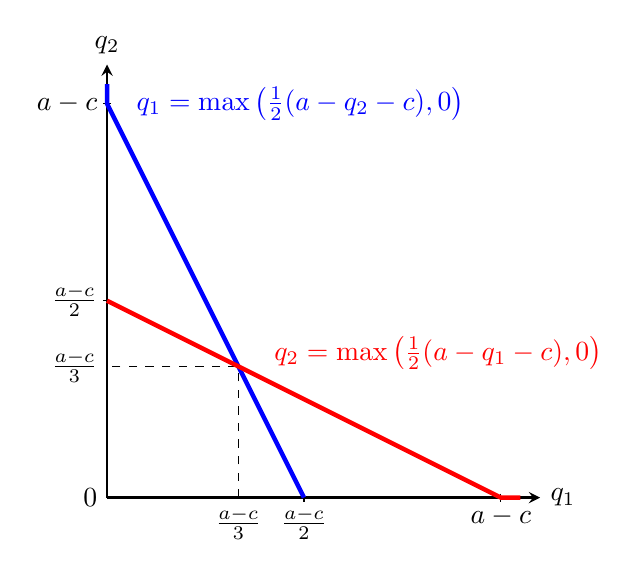
\begin{tikzpicture}[scale=5, >=stealth]

    % Axes
    \draw[->, thick] (0,0) -- (1.1,0) node[right] {$q_1$};
    \draw[->, thick] (0,0) -- (0,1.1) node[above] {$q_2$};

    % Axis Labels / Ticks
    \node[left] at (0,0) {$0$};
    \node[below] at (0.5,0) {$\frac{a-c}{2}$};
    \node[below] at (1,0) {$a-c$};
    \node[left] at (0,0.5) {$\frac{a-c}{2}$};
    \node[left] at (0,1) {$a-c$};

    % Tick marks
    \draw (0.5,0.01) -- (0.5,-0.01);
    \draw (1,0.01) -- (1,-0.01);
    \draw (0.01,0.5) -- (-0.01,0.5);
    \draw (0.01,1) -- (-0.01,1);

    % Dashed projection lines for Nash Equilibrium
    \draw[dashed] (1/3, 0) node[below] {$\frac{a-c}{3}$} -- (1/3, 1/3) -- (0, 1/3) node[left] {$\frac{a-c}{3}$};

    % Reaction Function 1 (Blue): q1 = max( (a - c - q2)/2 , 0 )
    % Vertical along q2-axis for q2 >= a-c, then down to q1 = (a-c)/2 at q2 = 0
    \draw[blue, ultra thick] (0, 1.05) -- (0, 1) -- (0.5, 0);

    % Reaction Function 2 (Red): q2 = max( (a - c - q1)/2 , 0 )
    % From q2 = (a-c)/2 at q1 = 0 down to q1 = a-c, then horizontal along q1-axis for q1 >= a-c
    \draw[red, ultra thick] (0, 0.5) -- (1, 0) -- (1.05, 0);

    % Legend / Function Labels
    \node[blue, right] at (0.05, 1) {$q_1 = \max \left( \frac{1}{2}(a - q_2 - c), 0 \right)$};
    \node[red, above right] at (0.4, 0.3) {$q_2 = \max \left( \frac{1}{2}(a - q_1 - c), 0 \right)$};

\end{tikzpicture}
\end{document}
